% Beamer slide template prepared by Tom Clark <tom.clark@op.ac.nz>
% Otago Polytechnic
% Dec 2012

\documentclass[10pt]{beamer}
\usetheme{Dunedin}
\usepackage{graphicx}
\usepackage{fancyvrb}
\usepackage{hyperref}

\newcommand\codeHighlight[1]{\textcolor[rgb]{1,0,0}{\textbf{#1}}}

\title{Introduction to DHCP}

\author[IN715]{Networks Three}
\institute[Otago Polytechnic]{
  Otago Polytechnic \\
  Dunedin, New Zealand \\
}
\date{}
\begin{document}

%----------- titlepage ----------------------------------------------%
\begin{frame}[plain]
  \titlepage
\end{frame}

\section{Overview}
%----------- frame  ----------------------------------------------%
\begin{frame}
  \frametitle{Basic Network Configuration}

  We generally configure hosts with a few standard items of network configuration.
  \begin{itemize}
    \item IP address
    \item Network mask
    \item Gateway address
    \item DNS server addresses
    \item Others:  syslog servers, proxy servers, NTP servers, etc.
  \end{itemize} 

  We don't want to do this manually if we have very many (i.e., more than one) host on our network.  We can use the Dynamic Host Configuration Protocol (DHCP) to manage this. 
\end{frame}



%----------- frame  ----------------------------------------------%
\begin{frame}
  \frametitle{DHCP Lease}
  \begin{itemize}
    \item The client outcome of the DHCP process is a \emph{Lease}.
    \item A lease is a package of configuration information that the client
          is allotted for a specified period of time.
  \end{itemize}  
\end{frame}


%----------- frame  ----------------------------------------------%
\begin{frame}
  \frametitle{DHCP Process}
  \begin{itemize}
    \item A DHCP client needing a lease begins by sending a DHCPDISCOVER to 
          the broadcast address, 255.255.255.255 with source address 0.0.0.0.
    \item DHCP servers respond to DHCPDISCOVER messages with DHCPOFFER messages. The offers contain suggested network configuration parameters.
    \item The client accepts one offer by sending a DHCPREQUEST message to 
          the offering server.
    \item The server responds with a DHCPACK containing the lease time and other parameters.  If the client request was flawed it responds with a DHCPNAK instead.
    \item The client checks that the proposed address is available by checking ARP.  If the address is already in use it complains to the server with a DHCPDECLINE message.
    \item The client may later renew or release the lease with a DHCPRENEW or DHCPRELEASE message.
  \end{itemize}  
\end{frame}

\begin{frame}
	\frametitle{DHCP Process}
	
	\includegraphics[scale=0.2]{DHCP_session.png}
	
	%Source: \url{https://commons.wikimedia.org/wiki/File:DHCP\_session.svg#/media/File:DHCP\_session.svg} Uploaded by Dsimic, CC-by-SA 4.0
\end{frame}




%----------- frame  ----------------------------------------------%
\begin{frame}
  \frametitle{DHCP Relay}
  \begin{itemize}
    \item Since the broadcast DHCPDISCOVER messages don't cross network
          boundaries, DHCP doesn't work across them.
    \item We get around this by running DHCP relay servers that relay
          DHCP messages to and from a central server.
  \end{itemize}  
\end{frame}


%----------- frame  ----------------------------------------------%
\begin{frame}
  \frametitle{DHCP Software}
  \begin{itemize}
    \item The ISC DHCP server package is the preferred server implementation 
          on *nix servers.
    \item Microsoft provides a server implementation for its server OSs.
  \end{itemize}  
\end{frame}

%----------- frame  ----------------------------------------------%
\begin{frame}
  \frametitle{Security Concerns}
  \begin{itemize}
    \item Rogue DHCP servers
    \item Unauthorised clients getting access to information
    \item Denial of Service by exhausting the address pool.
  \end{itemize}  
\end{frame}

\section{Basic configuration}
%----------- frame  ----------------------------------------------%
\begin{frame}
	\frametitle{Step 1: Plan}
	
	We need to answer the following questions:
	\begin{itemize}
		\item What is our overall network topology?
		\item On what networks will we serve DHCP?
		\item What are our service level requirements?
		\item For each network
		\begin{itemize}
			\item How many clients will we serve?
			\item What is their usage profile?
			\item Are there any machines that need static addresses?
		\end{itemize}
	\end{itemize}  
\end{frame}

%----------- frame  ----------------------------------------------%
\begin{frame}
	\frametitle{Planning, cont.}
	
	We also need specific information to serve to clients
	\begin{itemize}
		\item The location's domain name
		\item Client IP address ranges
		\item DNS server addresses
		\item Gateway addresses
		\item Subnet masks, broadcast addresses
		\item Possibly others
	\end{itemize}  
\end{frame}


%----------- frame  ----------------------------------------------%
\begin{frame}
	\frametitle{OpenBSD server setup}
	\begin{itemize}
		\item The ISC DHCP server, \emph{dhcpd}, is installed by default.
		\item The configuration file is \texttt{/etc/dhcpd.conf}
		\item We also need to enable the server by setting flags in \texttt{/etc/rc.conf.local}
	\end{itemize}  
\end{frame}

%----------- frame  ----------------------------------------------%
\begin{frame}
	\frametitle{A simple scenario}
	Suppose we have an OpenBSD server 
	\begin{itemize}
		\item connected to an external interface on 10.25.0.0/16
		\item connected to an internal interface on 192.168.1.0/24
		\item we want to serve DHCP on to clients on the internal network
	\end{itemize}  
	
	What goes in \texttt{dhcpd.conf}?
\end{frame}

\begin{frame}[fragile]
	\frametitle{Internal network with a static host}
	\begin{verbatim}
option domain-name "foo.org.nz";
option domain-name-servers 10.50.1.80, 10.50.1.82;
default-lease-time 86400;
max-lease-time 259200;
authoritative;

subnet 10.25.0.0 netmask 255.255.0.0 { }

subnet 192.168.1.0 netmask 255.255.255.0 {
    range 192.168.1.100  192.168.1.200;
    option routers 192.168.1.1;
    

    host bob {
        hardware ethernet 00:A0:78:6E:8E:A1;
        fixed-address 192.168.1.10;
    }
}
	
	\end{verbatim}
\end{frame}

%----------- frame  ----------------------------------------------%
\begin{frame}
	\frametitle{Global options}
	The first five lines specify global options that apply to every network
	we serve, unless overridden later.
\end{frame}
%----------- frame  ----------------------------------------------%
\begin{frame}
	\frametitle{Domain name}
	
	\texttt{ option domain-name "foo.org.nz"; }
	
	\vspace{5mm}
	This tells clients to append our domain name to unqualified hostnames, 
	i.e.  \texttt{ssh bar} goes to \texttt{bar.foo.bar.nz}.
\end{frame}
%----------- frame  ----------------------------------------------%
\begin{frame}
	\frametitle{DNS servers}
	
	\texttt{ option domain-name-servers 10.50.1.80, 10.50.1.82; }
	
	\vspace{5mm}
	Tell the clients to use these DNS servers for resolving.
	
\end{frame}

%----------- frame  ----------------------------------------------%
\begin{frame}
	\frametitle{Lease times}
	
	\texttt{ default-lease-time 86400 }
	
	\vspace{5mm}
	\texttt{ max-lease-time 259200 }
	
	\vspace{5mm}
	By default, our clients get a one day lease.  They can request a longer one,
	and we will allow up to three days.
	
	
\end{frame}
%----------- frame  ----------------------------------------------%
\begin{frame}
	\frametitle{Authoritative}
	
	\texttt{ authoritative; }
	
	\vspace{5mm}
	Our server is the authoritative source of network configuration on its networks. If a client request a lease renewal that this server does not recognise, it will direct the client to drop that lease and obtain a new one.
	
\end{frame}
%----------- frame  ----------------------------------------------%
\begin{frame}
	\frametitle{Networks}
	
	Next, we create a configuration block for every network.  There are network-specific options, and we can override global options.
\end{frame}
%----------- frame  ----------------------------------------------%
\begin{frame}[fragile]
	\frametitle{External network}
	\begin{verbatim}
	subnet 10.25.0.0 netmask 255.255.0.0 {}
	\end{verbatim}  
	
	Even though we won't serve DHCP on this subnet, it's good practice to 
	create an empty block for it.  Since it's directly connected to the server,
	dhcpd should know about it.
	
\end{frame}

%----------- frame  ----------------------------------------------%
\begin{frame}[fragile]
	\frametitle{Internal network}
	\begin{verbatim}
	subnet 192.168.1.0 netmask 255.255.255.0 {
	range 192.168.1.100 - 192.168.1.200;
	option routers 192.168.1.1;
	\end{verbatim}
	
	We will issue clients addresses in teh above range and direct them to use \texttt{192.168.1.1} as their default gateway.
\end{frame}
	
	%----------- frame  ----------------------------------------------%
	\begin{frame}[fragile]
		\frametitle{A Static Host}
		\begin{verbatim}
		
		host bob {
		    hardware ethernet 00:A0:78:6E:8E:A1;
		    fixed-address 192.168.1.10;
		}
		
		\end{verbatim}  
		
		The host \texttt{bob} gets a fixed address based on the MAC address.    
		
	\end{frame}

\begin{frame}[fragile]
	\frametitle{Finished configuration}
	\begin{verbatim}
	option domain-name "foo.org.nz";
	option domain-name-servers 10.50.1.80, 10.50.1.82;
	default-lease-time 86400;
	max-lease-time 259200;
	authoritative;
	
	subnet 10.25.0.0 netmask 255.255.0.0 { }
	
	subnet 192.168.1.0 netmask 255.255.255.0 {
	    range 192.168.1.100  192.168.1.200;
	    option routers 192.168.1.1;
	
	
	    host bob {
	        hardware ethernet 00:A0:78:6E:8E:A1;
	        fixed-address 192.168.1.10;
	    }
	}
	
	\end{verbatim}
\end{frame}	

\begin{frame}
	Questions?
\end{frame}
\end{document}
